\documentclass{article}

\usepackage[a4paper, left=1.5cm, right=1.5cm, top=2cm, bottom=2cm]{geometry}

\usepackage{../../../../components/components} % <-- ton fichier .sty, avec toutes tes définitions

\usepackage{fancyhdr}


% Configuration des en-têtes et pieds de page
\pagestyle{fancy}
\fancyhf{} % reset tout

\fancyhead[L]{DL2 Math-Info AL3}
\fancyhead[C]{Groupes}
\fancyhead[R]{2025-2026}

\fancyfoot[L]{Ewen Rodrigues de Oliveira}
\fancyfoot[R]{\thepage}

\begin{document}

\docTitle{Chapitre 1 : Groupes}

\section{Loi de composition interne}

\definition{Soit \(E\) un ensemble. Une \textbf{loi de composition interne} sur \(E\) est une application \( * : E \times E \to E \) qui à tout couple \((x, y) \in E \times E\) associe un élément \(x * y \in E\).}
\theorem{Propriété}{Associativité}{false}{\(*\) est associative si \( \forall x, y, z \in E, (x * y) * z = x * (y * z)\).}
\theorem{Propriété}{Elément neutre}{false}{On dit que \(e \in E\) est un élément neutre si \( \forall x \in E, e * x = x * e = x\).}
\remark{L'élément neutre est unique. La démonstration découle du fait que si on prend deux éléments neutres \(e\) et \(e'\), on a \(e * e' = e\) et \(e * e' = e'\), donc \(e = e'\).}
\theorem{Propriété}{Symétrique}{false}{Soient \(a,b \in E\). On dit que \(b\) est symétrique (ou inverse, ou opposé) de \(a\) si \(a * b = b * a = e\), où \(e\) est l'élément neutre.}
\theorem{Propriété}{Commutativité}{false}{\(*\) est commutative si \( \forall x, y \in E, x * y = y * x\).}

\vocabulary{Notations typiques pour les lois de composition interne : \(+\), \(\times\), \(\cdot\), \(\circ\), etc.}
\section{Notions de groupe}
\subsection{Généralités}

\definition{Soit G un ensemble muni d'une loi de composition interne \( * \). On dit que \((G, *)\) est un \textbf{groupe} si les trois propriétés suivantes sont vérifiées : 
\begin{itemize}
    \item \( * \) est associative.
    \item Il existe un élément neutre \(e \in G\).
    \item Tout élément de \(G\) possède un symétrique dans \(G\).
\end{itemize}
Si \( * \) est en plus commutative, on dit que \((G, *)\) est un \textbf{groupe abélien}.}

%% Exemples et contres exemples de groupes

\example{
    \textbf{Exemples de groupes :}
    \begin{itemize}
        \item \((\mathbb{Z}, +)\) : l'ensemble des entiers avec l'addition.
        \item \((\mathbb{R}^*, \times)\), \((\mathbb{Q}^*, \times)\), \((\mathbb{C}^*, \times)\) : l'ensemble des réels, rationnels et complexes non nuls avec la multiplication.
        \item $\left( \{ \text{bijections } X \to X \mid X \text{ est un ensemble} \}, \circ \right)$ : l'ensemble des bijections d'un ensemble \(X\) dans lui-même avec la composition.
    \end{itemize}
    \textbf{Contre-exemples de groupes :}
    \begin{itemize}
        \item \((\mathbb{N}, +)\) : l'ensemble des entiers naturels avec l'addition (pas d'élément neutre dans \(\mathbb{N}\)).
    \end{itemize}
}

\vocabulary{
    \textbf{Systèmes de notations pour les groupes :}
    \begin{itemize}
        \item Système additif : on note le groupe \((G, +)\), l'élément neutre est noté \(0\) et le symétrique de \(x\) est noté \(-x\).
        \item Système multiplicatif : on note le groupe \((G, \times)\) ou \((G, \cdot)\), l'élément neutre est noté \(1\) et le symétrique de \(x\) est noté \(x^{-1}\).
    \end{itemize}
}
\theorem{Propriété}{Produit de lois}{true}{
Soient \((G_1, *_1)\) et \((G_2, *_2)\) deux groupes. On définit une loi de composition interne sur \(G_1 \times G_2\) par * : 
\[
(g_1, g_2) * (h_1, h_2) \mapsto (g_1 *_1 h_1, g_2 *_2 h_2)
\]
pour tout \((x_1, y_1), (x_2, y_2) \in G_1 \times G_2\). Alors \((G_1 \times G_2, *)\) est un groupe.\newline
}
\theorem{Proposition}{Produit cartésien}{false}{Soient \((G_1, *_1)\) et \((G_2, *_2)\) deux groupes. On définit une loi de composition interne sur \(G_1 \times G_2\) par * comme susdit. Alors l'ensemble \((G_1 \times G_2, *)\) est un groupe, appelé le \textbf{groupe produit} de \((G_1, *_1)\) et \((G_2, *_2)\).}
\noindent\textbf{Preuve:}
\begin{itemize}
    \item \textit{Associativité :} Soient \((g_1, g_2), (h_1, h_2), (k_1, k_2) \in G_1 \times G_2\).
    \begin{align*}
        ((g_1, g_2) * (h_1, h_2)) * (k_1, k_2) &= (g_1 *_1 h_1, g_2 *_2 h_2) * (k_1, k_2) \\
        &= ((g_1 *_1 h_1) *_1 k_1, (g_2 *_2 h_2) *_2 k_2) \\
        &= (g_1 *_1 (h_1 *_1 k_1), g_2 *_2 (h_2 *_2 k_2)) \quad (\text{par associativité dans } G_1 \text{ et } G_2) \\
        &= (g_1, g_2) * (h_1 *_1 k_1, h_2 *_2 k_2) \\
        &= (g_1, g_2) * ((h_1, h_2) * (k_1, k_2))
    \end{align*}

    \item \textit{Élément neutre :} Soient \(e_1\) et \(e_2\) les éléments neutres de \(G_1\) et \(G_2\) respectivement. Alors \((e_1, e_2)\) est l'élément neutre de \(G_1 \times G_2\) car pour tout \((g_1, g_2) \in G_1 \times G_2\), \((e_1, e_2) * (g_1, g_2) = (e_1 *_1 g_1, e_2 *_2 g_2) = (g_1, g_2)\) et \((g_1, g_2) * (e_1, e_2) = (g_1 *_1 e_1, g_2 *_2 e_2) = (g_1, g_2)\).
    \item \textit{Symétrique :} Soit \((g_1, g_2) \in G_1 \times G_2\). Comme \(G_1\) et \(G_2\) sont des groupes, il existe \(g_1^{-1} \in G_1\) et \(g_2^{-1} \in G_2\) tels que \(g_1 *_1 g_1^{-1} = e_1\) et \(g_2 *_2 g_2^{-1} = e_2\). Alors le symétrique de \((g_1, g_2)\) dans \(G_1 \times G_2\) est \((g_1^{-1}, g_2^{-1})\) car :
\end{itemize}
\theorem{Propriété}{Produit cartésien et commutativité}{true}{
    Si \((G_1, *_1)\) et \((G_2, *_2)\) sont des groupes abéliens, alors leur produit cartésien \((G_1 \times G_2, *)\) est aussi un groupe abélien.
}
\remark{On pourrait prendre plus de deux groupes et faire le produit cartésien de plusieurs groupes.}
\subsection{Sous-groupes}
\definition{Soit \((G, \cdot)\) un groupe \textit{(on utilise la notation multiplicative, mais cela fonctionne aussi en notation additive)}. Un \textbf{sous-groupe} de \(G\) est un sous-ensemble \(H \subseteq G\) tel que \((H, \cdot)\) est lui-même un groupe.}
\theorem{Propriété}{Lien entre sous-groupe et groupe}{true}{
    Un sous-groupe est lui-même un groupe pour la même loi de composition interne que le groupe dont il est issu.
}

\example{\((Z, +)\) est un sous-groupe de \((\mathbb{R}, +)\).}
\theorem{Proposition}{Sous-groupe}{false}{
    Soit \((H, \cdot)\) un sous-groupe de \((G, \cdot)\ \Leftrightarrow\) %% système
    \begin{itemize}
        \item \(H \neq \emptyset\) : 1
        \item \( \forall h, h' \in H, h \cdot h' \in H\) (stabilité par la loi) : 2
        \item \( \forall h \in H, \exists h^{-1} \in H\) (stabilité par l'inverse) : 3
    \end{itemize}
}

\noindent\textbf{Preuve:}
\begin{itemize}
    \item \(\Rightarrow\)/ : Si \(H\) est un sous-groupe de \(G\), alors par définition de groupe, \(H\) satisfait 1, 2 et 3.
    \item \(\Leftarrow\)/ : Supposons que \(H\) vérifie les trois conditions. Nous devons montrer que \((H, \cdot)\) est un groupe.
    \begin{itemize}
        \item \textit{Associativité :} La loi de composition interne sur \(H\) est la même que celle sur \(G\), donc elle est associative.
        \item \textit{Élément neutre :} Soit \(e\) l'élément neutre de \(G\). Comme \(H\) est non vide, \(\exists h_0\in H\) et par la condition 3, \(h_0^{-1} \in H\). Par la définition de l'élément neutre dans \(G\), on a \(h_0 \cdot h_0^{-1} = e\). Donc \(e \in H\).
        \item \textit{Symétrique :} Par la condition 3, pour tout \(h \in H\), son inverse \(h^{-1}\) appartient à \(H\).
    \end{itemize}
    Ainsi, toutes les propriétés d'un groupe sont satisfaites pour \(H\), donc \(H\) est un sous-groupe de \(G\).   
\end{itemize}

\example{
    \begin{itemize}
        \item \((G, \cdot)\) est un sous-groupe de lui-même.
        \item \(\{1\}\) est un sous-groupe de \(G\).
        \item \((Z, +)\) est un sous-groupe de \((\mathbb{R}, +)\).
    \end{itemize}
}

\theorem{Proposition}{Intersection}{false}{
    Soit \((H_i)_{i \in I}\) une famille de sous-groupes de \((G, \cdot)\). Alors l'intersection \(H = \bigcap_{i \in I} H_i\) est un sous-groupe de \(G\).
}

\noindent\textbf{Preuve:}\\
\carreaux{20}


\theorem{Corollaire}{Sous-groupe engendré}{false}{Soit \(X \subseteq G\). Considérons  \(H = \bigcap_{i \in I} H_i\). C'est un \textbf{sous-groupe de \(G\) engendré par \(X\)}.}
\definition{Soit \(g \in G\).\\
On a posé pour \(n\in \mathbb{Z}, g^n = \underbrace{g \cdot g \cdot ... \cdot g}_{n \text{ fois}}\) si \(n > 0\), \(g^0 = e\) (élément neutre) et \(g^n = \underbrace{g^{-1} \cdot g^{-1} \cdot ... \cdot g^{-1}}_{-n \text{ fois}}\) si \(n < 0\).\newline
On pose \(g^{\mathbb{Z}} = \{ g^n \mid n \in \mathbb{Z} \}\) : c'est \textbf{l'ensemble des itérés} de \(g\).}

\theorem{Proposition}{Sous-groupe engendré}{false}{
    On a que \(g^{\mathbb{Z}}\) est un sous-groupe de \(G\) engendré par \(g\).
}

\noindent\textbf{Preuve:}\\
\carreaux{10}

\remark{En notation additive, l'ensemble des itérés de \(g\) est noté \(\mathbb{Z}g = \{ ng \mid n \in \mathbb{Z} \}\).}

\definition{Si \(G = g^{\mathbb{Z}}\), on dit que \(G\) est monogène et que \(g\) est un générateur de \(G\).}
\example{
    \(\mathbb{Z}\) est monogène et engendré par \(1\).
}
\vocabulary{Un groupe est cyclique s'il est fini et monogène.}

\definition{Si le sous-groupe engendré par \(X\) est \(G\), on dit que \(X\) est un système de générateurs de \(G\).}

%% 10 septembre 2025
\subsection{Sous-groupes de \((\mathbb{Z}, +)\)}
\theorem{Proposition}{}{true}{
    Soit \(k \in \mathbb{Z}\). On pose \(k\mathbb{Z} = \{ kn \mid n \in \mathbb{Z} \}\).
    On a que \(k\mathbb{Z}\) est un sous-groupe de \((\mathbb{Z}, +)\) engendré par \(k\).
}

\remark{
    \(k\mathbb{Z}\) = \(\langle k\rangle\) pour la loi +.
}

\theorem{Théorème}{}{false}{
    Soit \((H, +)\) un sous-groupe de \((\mathbb{Z}, +)\). Alors \(\exists !k \in \mathbb{N}\) tel que \(H = k\mathbb{Z}\).
}

\remark{Cela veut dire que tout sous-groupe de \((\mathbb{Z}, +)\) est de la forme \(k\mathbb{Z}\) pour un certain \(k \in \mathbb{N}\).}
\newpage
\noindent\textbf{Preuve:}\\
\carreaux{20}

\section{Relations d'équivalence et classes d'équivalence}

\definition{Soit \(E\) un ensemble. Soit \(R\) (un sous-ensemble de \(E \times E\)) une relation.\\
On pose \(xRy \Leftrightarrow (x, y) \in R\) et on dit que \(x\) est en relation avec \(y\) par \(R\).}
\theorem{Propriété}{Relation d'équivalence}{true}{
    Soit \(R\) une relation sur \(E\). On dit que \(R\) est une \textbf{relation d'équivalence} si :
    \begin{itemize}
        \item \(R\) est réflexive : \( \forall x \in E, xRx\).
        \item \(R\) est symétrique : \( \forall x, y \in E, xRy \Rightarrow yRx\).
        \item \(R\) est transitive : \( \forall x, y, z \in E, (xRy \wedge  yRz) \Rightarrow xRz\).
    \end{itemize}
}


\definition{Soit \(R\) une relation d'équivalence sur \(E\). Pour \(x \in E\), on appelle \textbf{classe d'équivalence} de \(x\) et on note \(\overline{x}\) (ou \([x]_R\) ou \(x+k\mathbb{Z}\)) l'ensemble \(\{ y \in E \mid xRy \}\).}


\theorem{Proposition}{}{true}{Si deux classes d'équivalence ont un élément en commun, alors elles sont égales.}

\definition{Soit \((F_i)_{i \in I}\) une famille de parties de \(E\). On dit que cette famille est une \textbf{partition} de \(E\) si :
\begin{itemize}
    \item \(E = \bigcup_{i \in I} F_i\) (la réunion des \(F_i\) est \(E\)).
    \item \( \forall i, j \in I, i \neq j \Rightarrow F_i \cap F_j = \emptyset\) (les \(F_i\) sont deux à deux disjointes).
\end{itemize}}
\newpage
\illustration{On peut reprendre l'idée intuitive d'un univers en probabilités :

    \begin{center}
        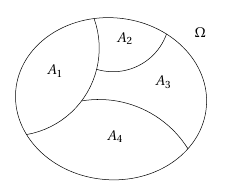
\includegraphics[width=0.25\textwidth]{./images/partition.png}
        \captionof{figure}{Partition de \(\Omega\) en \(A_1, A_2, A_3, A_4\)}
    \end{center}
}
\theorem{Proposition}{}{false}{Les classes d'équivalence d'une relation d'équivalence \(R\) forment une partition de \(E\).}
\noindent{
    \textbf{Preuve:}
    \begin{itemize}
        \item Les classes sont non vides.
        \item Deux classes différentes sont disjointes (elles n'ont pas d'élément en commun).
        \item L'union des classes est \(E\). $\Box$ 
    \end{itemize}
}

\theorem{Proposition}{}{false}{
    Soit \((F_i)_{i \in I}\) une partition de \(E\). On peut définir une relation d'équivalence \(R\) sur \(E\) par : \(xRy \Leftrightarrow \exists i \in I : x,y\in F_i\).\\
    Alors \(R\) est d'équivalence.
}

\noindent\textbf{Preuve:}\\
\begin{itemize}
    \item \textit{Réflexivité :} Soit \(x \in E\). Par définition de partition, \(\exists i \in I\) tel que \(x \in F_i\). Donc \(xRx\).
    \item \textit{Symétrie :} Soient \(x, y \in E\) tels que \(xRy\). Par définition de \(R\), \(\exists i \in I\) tel que \(x, y \in F_i\). Donc \(y, x \in F_i\) et ainsi \(yRx\).
    \item \textit{Transitivité :} Soient \(x, y, z \in E\) tels que \(xRy\) et \(yRz\). Par définition de \(R\), \(\exists i, j \in I\) tels que \(x, y \in F_i\) et \(y, z \in F_j\). Comme \(y \in F_i\) et \(y \in F_j\), on a \(F_i \cap F_j \neq \emptyset\). Par définition de partition, on en déduit que \(i = j\). Donc \(x, z \in F_i\) et ainsi \(xRz\). $\Box$
\end{itemize}

\definition{
    Soit \(R\) une relation d'équivalence sur \(E\).\\
    On appelle \textbf{ensemble quotient} de \(E\) par \(R\) et on note \(E/R\) l'ensemble des classes d'équivalence de \(R\).\\
    \textit{i.e.  \(E/R = \{ \overline{x} \mid x \in E \}\).}
}

\definition{
    Soit \(f : E \to F\) une application. \\
    On dit que f \textbf{passe au quotient} si \( \forall x, y \in E \text{ avec } xRy \Rightarrow f(x) = f(y)\).
}

\definition{
    Soit \(S \subseteq E\). On dit que \(S\) est un \textbf{système de représentants} pour \(R\) si pour toute classe \(C\) de \(R\), il existe un unique élément dans \(S \cap C\).
}

\section{Congruences}

\subsection{Rappels et généralités}

\definition{Soit \(k \in \mathbb{Z}\). 
On pose la relation \(\equiv_k\) sur \(\mathbb{Z}\) définie par : \(x \equiv_k y \Leftrightarrow y - x \in k\mathbb{Z}\) (i.e. \(k\) divise \(y - x\)).\\
On écrit aussi \(x \equiv y [k]\). \textit{i.e. \(\exists n \in \mathbb{Z}, y - x = kn\)}.
}

\vocabulary{
    \(\equiv_k\) est appelée \textbf{congruence modulo \(k\)}.
}

\theorem{Proposition}{Equivalence}{false}{
    \(\equiv_k\) est une relation d'équivalence sur \(\mathbb{Z}\).
}

\noindent\textbf{Preuve:}\\
\carreaux{10}


\theorem{Proposition}{\(\mathbb{Z}/k\mathbb{Z}\)}{false}{
    On a que \(\mathbb{Z}/\equiv_k = \{ \overline{0}, \overline{1}, \overline{2}, ..., \overline{k-1} \}\) noté \(\mathbb{Z}/k\mathbb{Z}\).\\

    En particulier, \{0, 1, 2, ..., k-1\} est un système de représentants pour \(\equiv_k\).
}
\noindent{
    \textbf{Preuve:}\\
    Soit \(x \in \mathbb{Z}\).\\
    Par la division euclidienne, \(\exists ! (q, r) \in \mathbb{Z} \times \{0, 1, 2, ..., k-1\}\) tel que \(x = kq + r\). Donc \(x - r = kq \in k\mathbb{Z}\) et ainsi \(x \equiv_k r\).\\
    Il reste à voir que \(\overline{i} \neq \overline{j}\) si \(i\neq j\) avec \(i, j \in \{0, 1, 2, ..., k-1\}\).\\
    En effet, \(i-j \in \{ 1-k, 2-k, ..., -1, 1, 2, ..., k-1 \}\) et \(i-j \neq 0\). \\
    Donc \(i-j \notin k\mathbb{Z}\) et ainsi \(i \not\equiv_k j\) donc \(\overline{i} \neq \overline{j}\). $\Box$
}

\theorem{Lemme}{}{false}{
    Soient \(x,y\in \mathbb{Z}\).\\
    Considérons \(\overline{x+y} \in \mathbb{Z}/k\mathbb{Z}\). Alors \(\overline{x+y}\) ne dépend que de \(\overline{x}\) et \(\overline{y}\).\\
    Autrement dit : \(\mathbb{Z} \to \mathbb{Z}/k\mathbb{Z}, x \mapsto \overline{x+y} \text{ et } y \mapsto \overline{x+y}\) passent au quotient.
}
\noindent\textbf{Preuve:}\\
\carreaux{10}


\theorem{Théorème}{\(\mathbb{Z}/k\mathbb{Z}\)}{false}{
On a que \((\mathbb{Z}/k\mathbb{Z}, +)\) est un groupe abélien. 
}
\newpage
\noindent\textbf{Preuve:}\\
\carreaux{7}

\theorem{Proposition}{\(\mathbb{Z}/k\mathbb{Z}\)}{false}{
Le groupe \((\mathbb{Z}/k\mathbb{Z}, +)\) est le groupe des entiers modulo \(k\).
}
\theorem{Proposition}{\(\mathbb{Z}/k\mathbb{Z}\)}{false}{
Le groupe \((\mathbb{Z}/k\mathbb{Z}, +)\) est cyclique et engendré par \(\overline{1}\).
}

\noindent{\textbf{Preuve:}\\
Le sous-groupe engendré par \(\overline{1}\) est \(\{ \overline{n} \mid n \in \mathbb{Z} \} = \{\overline{n\cdot 1} \mid n \in \mathbb{Z} \} = \mathbb{Z}/k\mathbb{Z}\). $\Box$
}

    \end{document}